\chapter{Appendix}

\vspace*{\fill}

\textit{Note : All code used in this thesis has been made available online via github - \url{https://github.com/sbmkvp/phd-thesis}.}

\cleardoublepage

%==============================================================================%
\section{Manual Counting}
%==============================================================================%

%-------------------------------------------------------------------------------
\subsection{Node.js App} \label{appendix:manualcount}
%-------------------------------------------------------------------------------
\vspace{1em}
\inputminted{javascript}{tools/manual-count/package.json}
\inputminted{javascript}{tools/manual-count/manualcount.js}

%-------------------------------------------------------------------------------
\subsection{Android App} \label{appendix:clicker}
%-------------------------------------------------------------------------------
\vspace{1em}
The Android manifest which defines the whole application along with the permissions it needs to function.
\inputminted{xml}{tools/clicker/manifest.xml}
\vspace{1em}
The layout of the app.
\inputminted{xml}{tools/clicker/layout.xml}
\vspace{1em}
The main logic of the app.
\inputminted{java}{tools/clicker/activity.java}
\pagebreak

%==============================================================================%
\section{Pilot Study}
%==============================================================================%

%-------------------------------------------------------------------------------
\subsection{Sensor} \label{appendix:pilot:sensor}
%-------------------------------------------------------------------------------
\vspace{1em}
\inputminted{javascript}{tools/pilot-study/sensor-package.json}
\inputminted{javascript}{tools/pilot-study/sensor-collect.js}
\inputminted{bash}{tools/pilot-study/sensor-collect.sh}

%-------------------------------------------------------------------------------
\subsection{Server} \label{appendix:pilot:server}
%-------------------------------------------------------------------------------
\vspace{1em}
\inputminted{javascript}{tools/pilot-study/server-package.json}
\inputminted{javascript}{tools/pilot-study/server-server.js}

%==============================================================================%
\section{Data Pipeline}\label{appendix:data:pipeline}
%==============================================================================%

\subsection{Sample configuration file } 
%-------------------------------------------------------------------------------
\vspace{1em}
\inputminted{javascript}{tools/pipeline/config_sample.json}

\subsection{Data Pipeline}
%-------------------------------------------------------------------------------
\vspace{1em}
\inputminted{bash}{tools/pipeline/pipeline}

\subsection{Daily Download}
%-------------------------------------------------------------------------------
\vspace{1em}
\inputminted{bash}{tools/pipeline/daily}

\subsection{Batch Download}
%-------------------------------------------------------------------------------
\vspace{1em}
\inputminted{bash}{tools/pipeline/batch}

\subsection{Component Scripts}
%-------------------------------------------------------------------------------
\vspace{1em}
Download the data from Azure data store.
\inputminted{bash}{tools/pipeline/scripts/download}
Transform the JSON files to CSV.
\inputminted{bash}{tools/pipeline/scripts/flatten}
Hash the MAC address field.
\inputminted{R}{tools/pipeline/scripts/hash}
Find the locations of the sensors.
\inputminted{bash}{tools/pipeline/scripts/locate}
Aggregate the counts based on MAC addresses.
\inputminted{R}{tools/pipeline/scripts/count}
Adjust the local counts based on probes to MAC ratio.
\inputminted{R}{tools/pipeline/scripts/adjust}
Impute missing values using Kalman filter.
\inputminted{R}{tools/pipeline/scripts/impute}
Download and update meta data.
\inputminted{bash}{tools/pipeline/scripts/meta_data}
Rotate the salt value in the configuration file.
\inputminted{bash}{tools/pipeline/scripts/rotate_salt}

\subsection{SQL queries}
%-------------------------------------------------------------------------------
\vspace{1em}
Manual counts.
\inputminted{sql}{tools/pipeline/queries/calibrations}
Device information.
\inputminted{sql}{tools/pipeline/queries/devices}
Location information.
\inputminted{sql}{tools/pipeline/queries/locations}
Installation notes.
\inputminted{sql}{tools/pipeline/queries/installs}

%==============================================================================%
\section{Benchmarking Data Tookit} \label{appendix:benchmark}
%==============================================================================%

This section documents all the code that has been used in the research.
The programming languages used are including but not limited to R, Bash, JavaScript and SQL.

%-------------------------------------------------------------------------------
\subsection{Simple implementation in R}
%-------------------------------------------------------------------------------
This R script lists all files in a given folder, parses them as JSON data serially, aggregates the records for each time interval and finally writes it to disk as a CSV file.
\vspace{1em}
\inputminted{R}{analysis/data-toolkit/old-toolkit.r}

%-------------------------------------------------------------------------------
\subsection{Serial implementation in bash}
%-------------------------------------------------------------------------------
This bash script lists all the files in a given folder, parses them into JSON data \textit{serially}, aggregates the resulting records for each time interval and finally writes it to disk as a CSV file.
\vspace{1em}
\inputminted{bash}{analysis/data-toolkit/new-toolkit.sh}

%-------------------------------------------------------------------------------
\subsection{Parallel implementation in bash}
%-------------------------------------------------------------------------------

This bash script lists all the files in a given folder, parses them into JSON data \textit{in parallel}, aggregates the resulting records for each time interval and finally writes it to disk as a CSV file.
\vspace{1em}
\inputminted{bash}{analysis/data-toolkit/new-toolkit-parallel.sh}
\pagebreak

%===============================================================================
\section{Sample Probe Request} \label{appendix:sampleprobe}
%===============================================================================
This is a sample probe request captured using tshark and saved in the JSON format.

\vspace{1em}
\inputminted{javascript}{analysis/data-collection/samplepacket.json}
\pagebreak

%==============================================================================%
\section{Opensource software used}\label{appendix:software}
%==============================================================================%

This section provides a non-exhaustive list of the key open-source/free software that have been used in this research.

\begin{itemize}
  \item \textbf{R project for statistical computing}
    \begin{itemize}
      \item \textbf{tidyverse}
      \item \textbf{imputeTS}
      \item \textbf{tmap}
      \item \textbf{lubridate}
      \item \textbf{ggplot2}
      \item \textbf{classInt}
      \item \textbf{Cairo}
      \item \textbf{fmsb}
      \item \textbf{digest}
      \item \textbf{ggrepel}
      \item \textbf{ggridges}
      \item \textbf{maptools}
      \item \textbf{tidyquant}
      \item \textbf{treemapify}
      \item \textbf{sf}
      \item \textbf{RJSONIO}
      \item \textbf{rgdal}
      \item \textbf{rgeos}
      \item \textbf{viridis}
      \item \textbf{xtable}
      \item \textbf{scales}
      \item \textbf{showtext}
      \item \textbf{reshape2}
      \item \textbf{rmarkdown}
    \end{itemize}
  \item \textbf{Python}
  \item \textbf{PHP}
  \item \textbf{Javascript}
    \begin{itemize}
      \item \textbf{node.js}
      \item \textbf{socket.io}
      \item \textbf{moment.js}
      \item \textbf{pm2}
      \item \textbf{express}
      \item \textbf{Data Driven Documents}
      \item \textbf{jQuery}
      \item \textbf{Bootstrap}
      \item \textbf{highcharts}
    \end{itemize}
  \item \textbf{GNU/Linux}
    \begin{itemize}
      \item \textbf{Archlinux}
      \item \textbf{CentOS}
      \item \textbf{Debian}
      \item \textbf{Ubuntu}
      \item \textbf{AlpineOS}
    \end{itemize}
  \item \textbf{git}
  \item \textbf{imagemagik}
  \item \textbf{ffmpeg}
  \item \textbf{fzf}
  \item \textbf{ripgrep}
  \item \textbf{Postgres}
  \item \textbf{PostGIS}
  \item \textbf{QGIS}
  \item \textbf{gdal}
  \item \textbf{geos}
  \item \textbf{igraph}
  \item \textbf{Python}
  \item \textbf{Android }
  \item \textbf{vim}
  \item \textbf{Latex}
  \item \textbf{jq}
  \item \textbf{Apache}
  \item \textbf{nginx}
  \item \textbf{OpenJDK}
  \item \textbf{Wireshark}
  \item \textbf{OpenSSH}
  \item \textbf{OpenSSL}
  \item \textbf{GNUPG}
  \item \textbf{Libreoffice}
  \item \textbf{RaspberryPi}
  \item \textbf{Docker}
  \item \textbf{termux}
  \item \textbf{OpenStreetMap}
  \item \textbf{Leaflet}
\end{itemize}

%===============================================================================
% \chapter{Research Article}
%===============================================================================
% 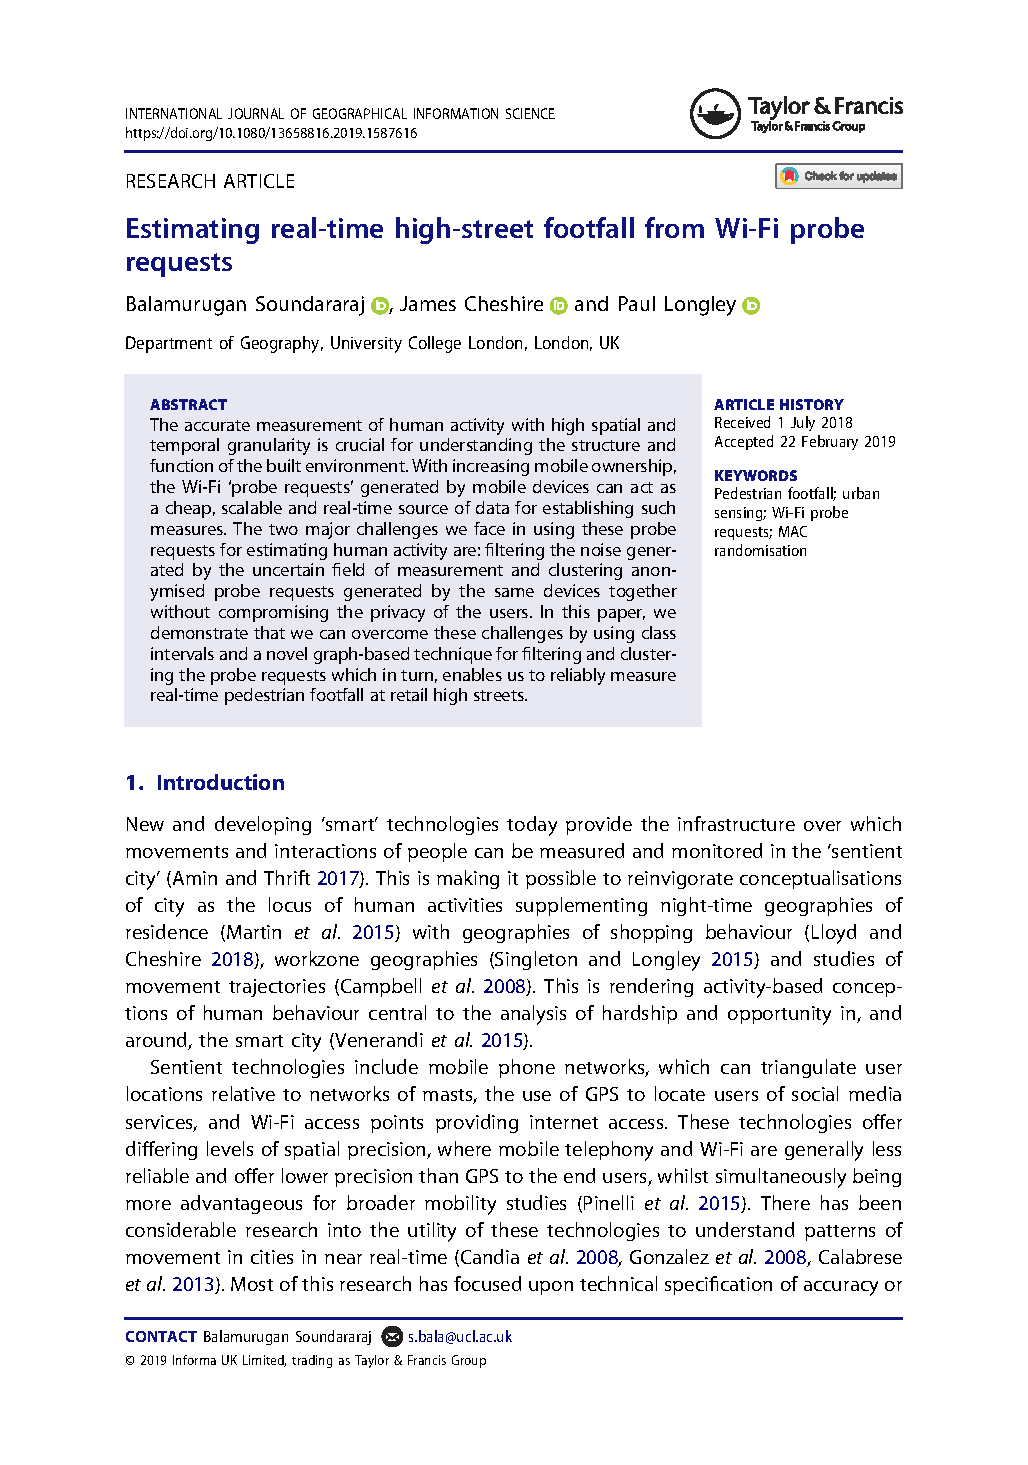
\includepdf[pages=1-15]{documents/ijgis-paper.pdf}
